\documentclass[12pt,letterpaper]{article}

% ---------- Standard setup ----------
\usepackage[margin=1in]{geometry}
\usepackage{amsmath,amssymb,amsthm}
\usepackage{bm}
\usepackage{graphicx}
\usepackage{tikz}
\usepackage{enumitem}
\setlist[itemize]{itemsep=2pt,topsep=2pt}
\setlist[enumerate]{itemsep=2pt,topsep=2pt}

\newtheorem{proposition}{Proposition}
\newtheorem{lemma}{Lemma}
\newtheorem{claim}{Claim}

\setlength{\parindent}{0pt}
\setlength{\parskip}{4pt}

% ---------- Header ----------
\begin{document}

\begin{center}
  {\large\bfseries ECON 6000 -- Microeconomics I}\\[4pt]
  {\large\bfseries Assignment 1}\\[10pt]
  Name: xingming\\
  Student ID: 1432037
\end{center}

\vspace{6pt}

% ==========================================================
\section*{Question 1}

We have $L=2$, $x(p,w)$ is single-valued, and $x(p,w)$ satisfies Walras' law and WARP.

\subsection*{1.1}

Yes, the Slutsky matrix, $S$, is symmetric when $L=2$. Since there are only 2 commodities, we end up with a $2\times 2$ Slutsky matrix, so to prove symmetry of $S$ we essentially need to prove $S_{12}= S_{21}$.

Firstly, since $x(p,w)$ is single-valued and we assume it is differentiable, all the derivatives below exist, so the Slutsky matrix is well defined. Also, $x(p,w)$ is homogeneous of degree 0 by Walras' law and the Weak Axiom of Revealed Preference. If the function is homogeneous of degree 0, we can later apply the results from Prop.~2.E.1. Let's write down the $(l,k)$th entry of $S$:
\[
S_{lk}(p,w)
= \frac{\partial x_l(p,w)}{\partial p_k}
+ \frac{\partial x_l(p,w)}{\partial w}\, x_k(p,w).
\]

\textit{Step 1 (rows).} Multiplying by $p_k$,
\[
S_{lk}\,p_k
= \frac{\partial x_l(p,w)}{\partial p_k}\,p_k
+ \frac{\partial x_l(p,w)}{\partial w}\, x_k(p,w)\,p_k .
\]
Summing across $k$ and applying the result from Prop.~2.E.1 (homogeneity of degree 0, which we get from WARP and Walras' law), we obtain
\begin{align*}
\sum_k S_{lk}\,p_k
&= \sum_k \frac{\partial x_l(p,w)}{\partial p_k}\,p_k
 + \frac{\partial x_l(p,w)}{\partial w}\sum_k x_k(p,w)\,p_k \\
&= \sum_k \frac{\partial x_l(p,w)}{\partial p_k}\,p_k
 + \frac{\partial x_l(p,w)}{\partial w}\,w = 0,
\end{align*}
where the second line uses Walras' law, $\sum_k p_k x_k(p,w) = w$. Hence
\[
S_{l1}p_1 + S_{l2}p_2 = 0 \qquad \forall\, l=1,2 .
\]
In particular, for $l=1$:
\[
S_{11}p_1 + S_{12}p_2 = 0 \;\Longrightarrow\; S_{12} = \frac{-S_{11}p_1}{p_2}.
\]

\textit{Step 2 (columns).} Next, multiplying by $p_l$,
\[
p_l\, S_{lk}(p,w)
= \frac{\partial x_l(p,w)}{\partial p_k}\,p_l
+ \frac{\partial x_l(p,w)}{\partial w}\, x_k(p,w)\,p_l .
\]
Summing over all goods $l$ and applying Props.~2.E.2 and 2.E.3 (both follow from differentiating Walras' law),
\begin{align*}
\sum_l S_{lk}(p,w)\,p_l
&= \sum_l \frac{\partial x_l(p,w)}{\partial p_k}\,p_l
 + x_k(p,w)\sum_l \frac{\partial x_l(p,w)}{\partial w}\,p_l \\
&= \underbrace{-x_k(p,w)}_{(1)} + \underbrace{x_k(p,w)}_{(2)} = 0
\qquad \forall\, k=1,2 .
\end{align*}
\begin{itemize}
  \item (1) comes from Prop.~2.E.2 (Cournot aggregation):
  $\displaystyle\sum_l p_l\frac{\partial x_l(p,w)}{\partial p_k} + x_k(p,w) = 0$, i.e.\
  $\displaystyle\sum_l p_l\frac{\partial x_l(p,w)}{\partial p_k} = -x_k(p,w)$.
  \item (2) comes from Prop.~2.E.3 (Engel aggregation):
  $\displaystyle\sum_l p_l\frac{\partial x_l(p,w)}{\partial w} = 1$.
\end{itemize}
Therefore $\sum_l S_{lk}\,p_l = 0$ for all $k=1,2$. In particular, for $k=1$:
\[
S_{11}p_1 + S_{21}p_2 = 0 \;\Longrightarrow\; S_{21} = \frac{-S_{11}p_1}{p_2} = S_{12}.
\]
Therefore the Slutsky matrix is symmetric for $L=2$.



\subsection*{1.2}

No, the proof does not extend to the case where $L=3$. Recall from 1.1 that
\[
S(p,w)\,p = 0 \quad (1) \qquad\text{and}\qquad S(p,w)^{T} p = 0 \quad (2).
\]
Taking the first row of each,
\begin{align*}
S_{11}p_1 + S_{12}p_2 + S_{13}p_3 &= 0 \qquad \text{from (1)} \quad (3)\\
S_{11}p_1 + S_{21}p_2 + S_{31}p_3 &= 0 \qquad \text{from (2)} \quad (4)
\end{align*}
Subtracting, $(3)-(4)$ gives
\[
(S_{12}-S_{21})\,p_2 + (S_{13}-S_{31})\,p_3 = 0 .
\]
Since $p_2, p_3 > 0$, we may have the case that
\[
S_{12}-S_{21} = p_3 \qquad\text{and}\qquad S_{13}-S_{31} = -p_2,
\]
so that $p_3p_2 - p_2p_3 = 0$. In this case $S_{12}\neq S_{21}$ and $S_{13}\neq S_{31}$. In $L=2$ there is only one term left, so the equation forces $S_{12}=S_{21}$; with two terms it no longer does. Therefore, the conditions from 1.1 no longer force symmetry, and the proof does not extend to $L=3$.

\subsection*{1.3}

SARP is just a stronger version of WARP that forbids preference reversal (also through indirect chains). According to Prop.~2.F.2, if $x(p,w)$ satisfies Walras' law and WARP, then $S(p,w)$ is negative semidefinite. Since SARP implies WARP, this holds under SARP as well. For $L=2$, we know from 1.1 that $S$ is also symmetric, so we agree with the statement. However, the argument does not stand for $L=3$. SARP still gives negative semidefiniteness through WARP, but by 1.2 the tools from Chapter 2 cannot deliver symmetry when $L=3$. So with only what we know from Chapter 2, we cannot conclude that the statement holds for $L=3$. This does not mean $S$ fails to be symmetric; we just cannot prove it here.

% ==========================================================
\section*{Question 2}

\subsection*{2.1}

Let $w^t = p^t\cdot x^t$ denote the wealth in year $t$, so $w^1=18$, $w^2=10$, $w^3=15$.

\textit{$x^1$ vs.\ $x^2$:}
\[
p^1\cdot x^2 = 15 < p^1\cdot x^1 = 18, \qquad p^2\cdot x^1 = 15 > p^2\cdot x^2 = 10 .
\]
So $x^1$ is revealed preferred to $x^2$, and not the other way around.

\textit{$x^3$ vs.\ $x^2$:}
\[
p^3\cdot x^2 = 10 < p^3\cdot x^3 = 15, \qquad p^2\cdot x^3 = 15 > p^2\cdot x^2 = 10 .
\]
So $x^3$ is revealed preferred to $x^2$.

\textit{$x^3$ vs.\ $x^1$:}
\[
p^3\cdot x^1 = 15 = p^3\cdot x^3, \qquad p^1\cdot x^3 = 27 > p^1\cdot x^1 = 18 .
\]
So $x^3$ is revealed preferred to $x^1$.

Hence $x^3$ is revealed preferred to $x^1$, $x^1$ is revealed preferred to $x^2$, and $x^3$ is revealed preferred to $x^2$. In every pair, the bundle that is revealed preferred is not affordable when the other bundle is chosen, so there is no preference reversal and WARP is satisfied.

\subsection*{2.2}

From the previous results, we already know $x^3 \succsim x^2$. Now we need to compare $x^4$ with $x^3$, and $x^4$ with $x^2$.

\textit{$x^4$ and $x^3$:}
\[
p^3\cdot x^3 = 15 > p^3\cdot x^4 = 14,
\]
then $x^3 \succsim x^4$. By monotonicity, we may find $x^5 = x^4 + (0.2,\,0.5) = (4.2,\,10.5) \gg x^4$, therefore $x^5 \succ x^4$. But
\[
p^3\cdot x^5 = 4.2\times 1 + 10.5\times 1 = 14.7 < w^3 = 15,
\]
so $x^3 \succsim x^5 \succ x^4 \;\Longrightarrow\; x^3 \succ x^4$.

\textit{$x^4$ and $x^2$:}
\[
p^2\cdot x^4 = 14 > w^2 = 10,
\]
so it's inconclusive from WARP. Since $x^3 \succsim x^2$, by convexity
\[
\bar{x} = \alpha x^3 + (1-\alpha)x^2 \succsim x^2, \qquad \alpha\in[0,1].
\]
Choose $\alpha$ so that $\bar{x}$ lies strictly below $x^4$ in both goods; $\alpha = 0.6$ works:
\[
\bar{x} = 0.4\,x^2 + 0.6\,x^3 = (3.8,\,9.2) \succsim x^2 .
\]
Since $x^4 = (4,10) \gg \bar{x}$, by monotonicity $x^4 \succ \bar{x}$, and then $x^4 \succ x^2$. By transitivity,
\[
x^3 \succ x^4 \succ x^2 .
\]
So $x^4$ is worse than $x^3$ but better than $x^2$.

\textit{With convexity only.} We may still conclude $x^3 \succsim x^4$ since $x^3$ is revealed preferred to $x^4$ (as $p^3\cdot x^4 < w^3$), and we may still say $\alpha x^3 + (1-\alpha)x^4 \succsim x^4$, but no further conclusion can be made without the monotonicity assumption. For $x^4$ and $x^2$, we may still say $\bar{x} = (3.8,\,9.2) \succsim x^2$. Even though $x^4 \gg \bar{x}$, without monotonicity we cannot conclude $x^4 \succ \bar{x} \succsim x^2$, so $x^4$ and $x^2$ cannot be compared. The comparison collapses.

\subsection*{2.3}

Now $x^4 = (4,10)$ is chosen at $p^4 = (2,1)$, so $w^4 = p^4\cdot x^4 = 18$. The expanded table is:

\begin{center}
\begin{tabular}{c|cccc}
 & $p^1=(1,2)$ & $p^2=(1,1)$ & $p^3=(1,1)$ & $p^4=(2,1)$ \\ \hline
$x^1=(12,3)$ & $\mathbf{18}$ & 15 & 15 & 27 \\
$x^2=(5,5)$  & 15 & $\mathbf{10}$ & 10 & 15 \\
$x^3=(3,12)$ & 27 & 15 & $\mathbf{15}$ & 18 \\
$x^4=(4,10)$ & 24 & 14 & 14 & $\mathbf{18}$
\end{tabular}
\end{center}

We can still obtain the previous results: $x^1$ is revealed preferred to $x^2$, $x^3$ is revealed preferred to $x^2$, and $x^3$ is revealed preferred to $x^1$.

\textit{Check $x^4$ with $x^3$:}
\[
p^3\cdot x^4 = 14 < w^3 = 15 \qquad\text{but}\qquad p^4\cdot x^3 = 18 = w^4 = p^4\cdot x^4 .
\]
So $x^3$ is revealed preferred to $x^4$, and $x^4$ is also revealed preferred to $x^3$. WARP is violated.

\textit{Check $x^4$ with $x^2$:}
\[
p^4\cdot x^2 = 15 < p^4\cdot x^4 = 18 \qquad\text{and}\qquad p^2\cdot x^4 = 14 > p^2\cdot x^2 = 10,
\]
so it has to be that $x^4$ is revealed preferred to $x^2$.

\textit{Check $x^4$ with $x^1$:} $p^4\cdot x^1 = 27 > w^4$ and $p^1\cdot x^4 = 24 > w^1$, so neither is revealed preferred to the other.

In summary, $x^1$ is revealed preferred to $x^2$, $x^3$ to $x^2$, $x^3$ to $x^1$, and $x^4$ to $x^2$. But $x^3$ is revealed preferred to $x^4$ and $x^4$ is also revealed preferred to $x^3$, so WARP is not satisfied.

% ==========================================================
\section*{Question 3}

We assume the standard non-negative consumption set $X=\mathbb{R}^2_+$, and
\[
u(x_1,x_2) = (x_1-1)(x_2-1).
\]

\subsection*{3.1}

\textit{Utility level 0.} $u(x_1,x_2)=0$ exactly when $x_1=1$ or $x_2=1$, so the indifference set is the two lines $x_1=1$ and $x_2=1$. The superior set $\{x : u(x)\ge 0\}$ consists of two pieces: the region where $x_1\ge 1$ and $x_2\ge 1$ (both factors non-negative), and the box $[0,1]^2$, where both factors are non-positive so their product is still non-negative. The two remaining regions ($x_1>1,\,x_2<1$ and $x_1<1,\,x_2>1$) give $u<0$. The hatched area below is the superior set.

\begin{center}
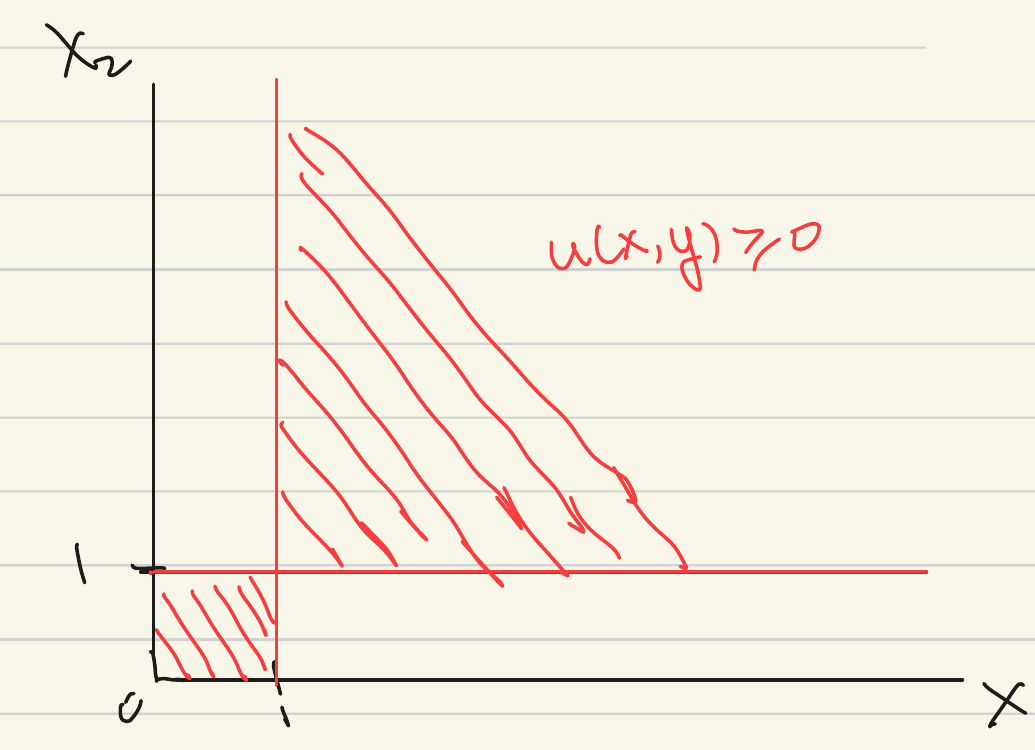
\includegraphics[width=0.45\textwidth]{figures/q3_1_u0.png}
\end{center}

\textit{Utility level 1.} When $u=1$,
\[
(x_1-1)(x_2-1)=1 \;\Longrightarrow\; x_2-1=\frac{1}{x_1-1} \;\Longrightarrow\; x_2 = \frac{1}{x_1-1}+1 = \frac{x_1}{x_1-1}.
\]
As $x_1\to\infty$, $x_2\to 1$, and as $x_1\to 1^+$, $x_2\to\infty$, so the curve has asymptotes $x_1=1$ and $x_2=1$ and passes through $(2,2)$. In addition, $u(0,0)=(-1)(-1)=1$, so the origin is also on this indifference set. It is the only such point in $[0,1]^2$, since there $(1-x_1)(1-x_2)<1$ unless $x_1=x_2=0$.

\begin{center}
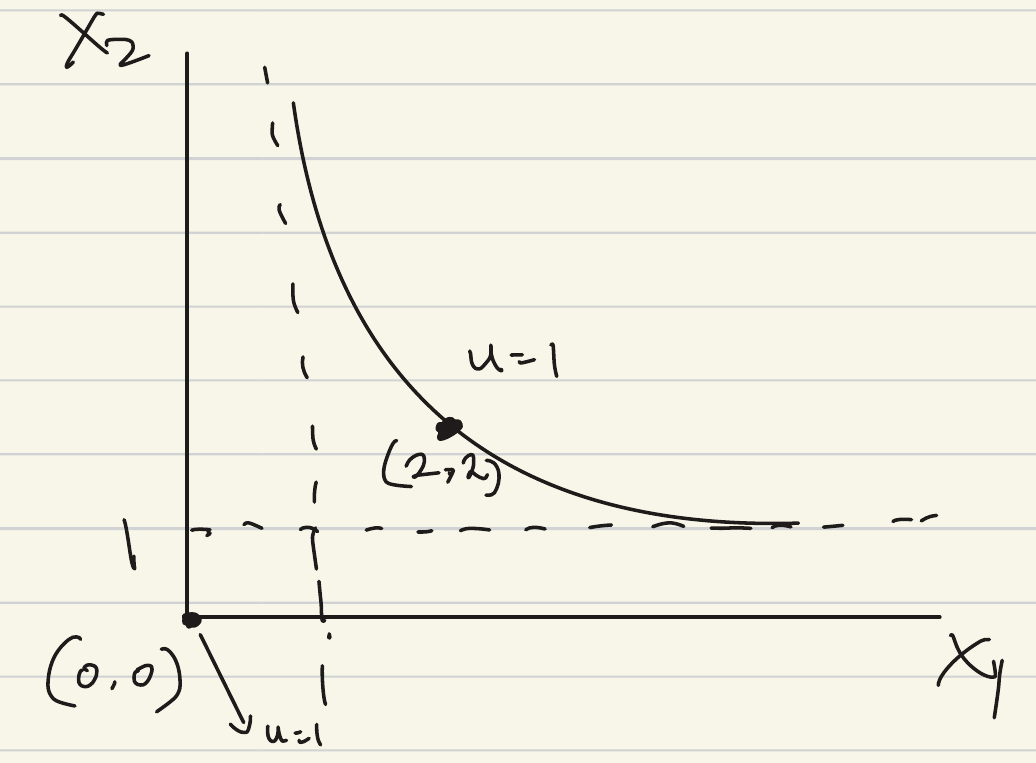
\includegraphics[width=0.45\textwidth]{figures/q3_1_u1.png}
\end{center}

\subsection*{3.2}

\textit{Not convex.} For a preference relation to be convex, every upper contour set $\{(x_1,x_2): (x_1-1)(x_2-1)\ge k\}$ must be convex. Take $k=1$ and consider the two points $(0,0)$ and $(2,2)$, both with $u=1$. Their convex combination
\[
0.5\,(0,0) + 0.5\,(2,2) = (1,1), \qquad u(1,1)=0 < 1 = u(0,0)=u(2,2),
\]
has a lower utility level, so $(1,1)$ is not in the upper contour set. Hence the upper contour set is not convex and the preferences are not convex.

\textit{Not locally non-satiated.} Take $x=(0,0)$ and any $0<\varepsilon<1$. For every $y\in B_\varepsilon(0,0)\cap\mathbb{R}^2_+$ with $y\neq(0,0)$ we have $0\le y_1,y_2<1$ with at least one strictly positive, so
\[
u(y) = (1-y_1)(1-y_2) < 1 = u(0,0).
\]
There is no bundle arbitrarily close to $(0,0)$ that is strictly preferred to it, so local non-satiation fails at $(0,0)$.

\textit{Not monotone.} Monotonicity implies local non-satiation, so the preferences cannot be monotone if they are not locally non-satiated. Directly: $(0.5,0.5)\gg(0,0)$ but $u(0.5,0.5)=0.25<1=u(0,0)$.

\subsection*{3.3}

Now
\[
v(x_1,x_2)=\begin{cases}(x_1-1)(x_2-1) & \text{if } x_1>1 \text{ and } x_2>1,\\ 0 & \text{otherwise (i.e.\ } x_1\le 1 \text{ or } x_2\le 1\text{)},\end{cases}
\]
with $x_1,x_2\ge 0$.

\textit{Utility level 0.} The indifference set $v=0$ is the whole region where $x_1\le 1$ or $x_2\le 1$ (red below), not just two lines. On the region $x\gg 1$ (blue) we have $v>0$. Therefore the superior set $\{x: v(x)\ge 0\}$ is the entire $\mathbb{R}^2_+$, as indicated by the arrow in the figure.

\begin{center}
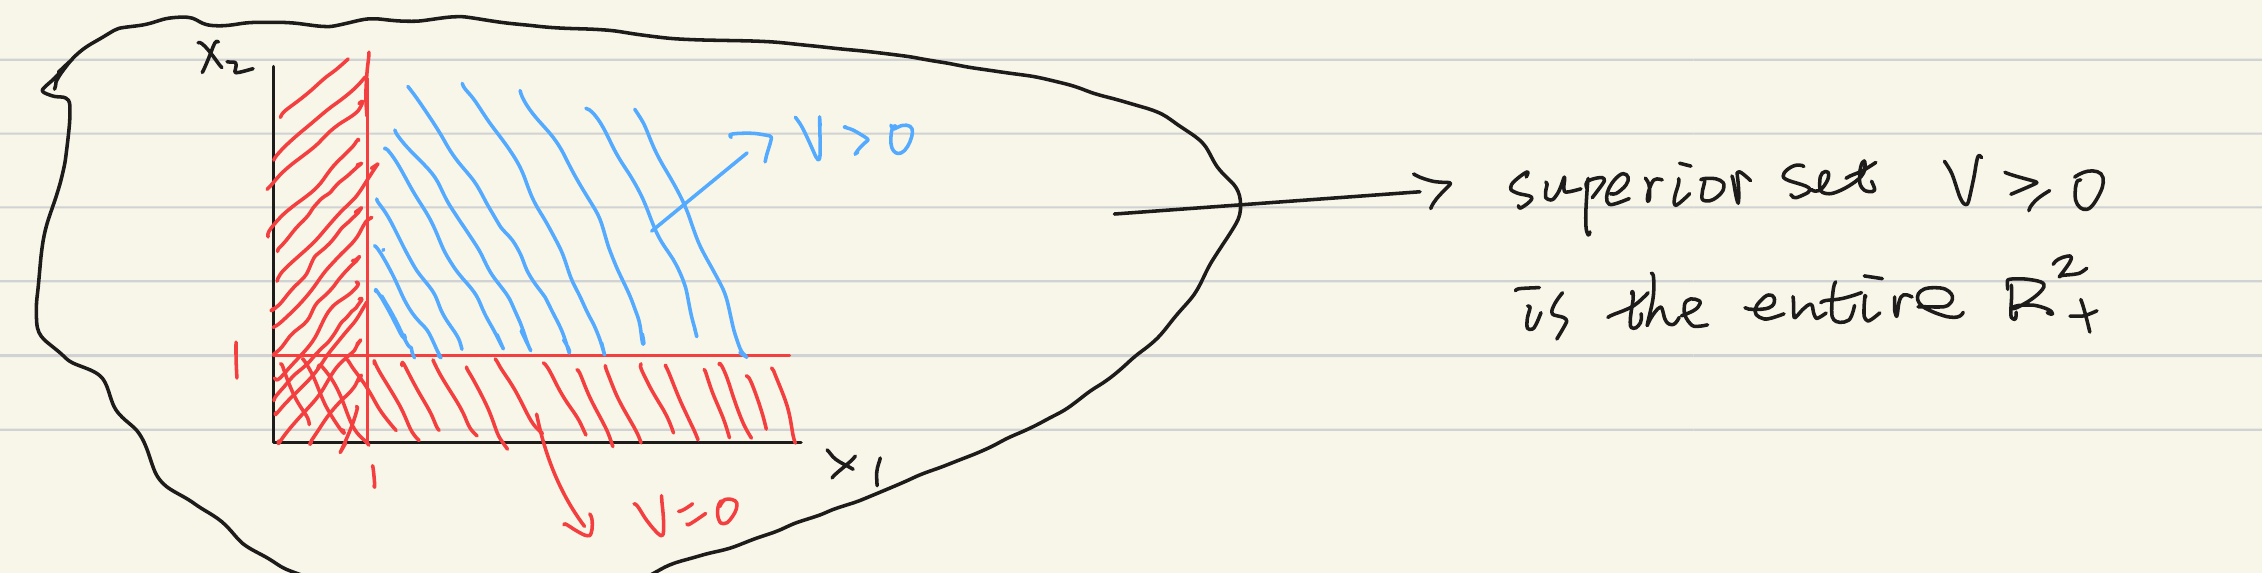
\includegraphics[width=0.75\textwidth]{figures/q3_3_v0.png}
\end{center}

\textit{Utility level 1.} When $v=1$ it must be the case that $x\gg 1$, and as before
\[
x_2 = \frac{x_1}{x_1-1}.
\]
The graph is the same as in 3.1 except that $(0,0)$ is no longer included, since $v(0,0)=0$. (The curve in the figure is $v=1$.)

\begin{center}
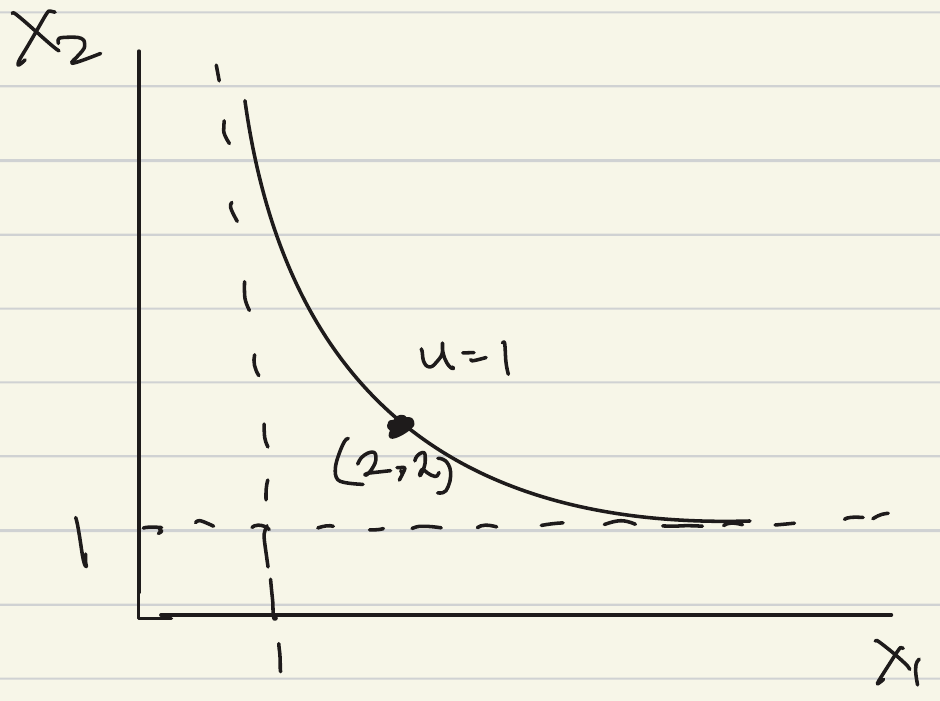
\includegraphics[width=0.4\textwidth]{figures/q3_3_v1.png}
\end{center}

\subsection*{3.4}

\textit{Convex.} The preference represented by $v$ is convex. For $k\le 0$, the upper contour set $\{x: v(x)\ge k\}$ is the entire $\mathbb{R}^2_+$, which is convex. For $k>0$, the upper contour set is
\[
\{x\in\mathbb{R}^2_+ : x\gg 1,\ (x_1-1)(x_2-1)\ge k\} = \Big\{x : x_1>1,\ x_2 \ge 1+\tfrac{k}{x_1-1}\Big\},
\]
the region on and above the upper hyperbola branch. The boundary $g(x_1)=1+\frac{k}{x_1-1}$ satisfies $g''(x_1)=\frac{2k}{(x_1-1)^3}>0$ for $x_1>1$, so it is a convex function, and the region above the graph of a convex function on the convex domain $x_1>1$ is a convex set. All upper contour sets are convex, so the preferences are convex.

\textit{Not locally non-satiated.} For $x=(0,0)$ and any $0<\varepsilon<1$, every $y\in B_\varepsilon(0,0)\cap\mathbb{R}^2_+$ has $y_1,y_2<1$, so $v(y)=0=v(0,0)$. No nearby bundle is strictly preferred, so local non-satiation fails.

\textit{Not monotone.} As before, this implies the preferences are not monotone. Directly: $(0.5,0.5)\gg(0,0)$ but $v(0.5,0.5)=0=v(0,0)$.

\subsection*{3.5}

We assume $p_1+p_2<w$, so $(1,1)$ is affordable, and ask whether the same bundle $x^*$ is optimal for both $v(x_1,x_2)$ and $u(x_1,x_2)$.

\textit{Starting with $v$.} At $(1,1)$ we only obtain $v(1,1)=0$. Since $p_1+p_2<w$, we may still increase both goods by a small amount so that $x_1,x_2>1$, which gives a strictly positive utility while remaining affordable. So the optimum lies in the region $x\gg 1$. There $v$ is strictly increasing in both arguments, so the budget constraint binds, and we solve
\[
\max_{x}\; v(x) = (x_1-1)(x_2-1) \qquad \text{s.t. } x\gg 1 \text{ and } p_1x_1+p_2x_2 = w .
\]
The Lagrangian is
\[
\mathcal{L}(x,\lambda) = (x_1-1)(x_2-1) + \lambda\,(w - p_1x_1 - p_2x_2),
\]
with first-order conditions
\[
\mathcal{L}_{x_1} = x_2-1-\lambda p_1 = 0, \qquad \mathcal{L}_{x_2} = x_1-1-\lambda p_2 = 0
\;\;\Longrightarrow\;\; \frac{x_2-1}{x_1-1} = \frac{p_1}{p_2}.
\]
So $(x_2-1)p_2 = (x_1-1)p_1$, i.e.\ $x_1 = \frac{(x_2-1)p_2}{p_1}+1$. From the budget constraint, $x_1 = \frac{w-p_2x_2}{p_1}$. Setting these equal,
\[
w - p_2x_2 = (x_2-1)p_2 + p_1 \;\Longrightarrow\; 2p_2x_2 = w+p_2-p_1 \;\Longrightarrow\; x_2^* = \frac{w+p_2-p_1}{2p_2},
\]
and similarly
\[
x_1^* = \frac{w+p_1-p_2}{2p_1}.
\]
Both exceed 1 because $w>p_1+p_2$. The maximized utility is
\begin{align*}
v(x^*) = (x_1^*-1)(x_2^*-1)
&= \left(\frac{w+p_1-p_2}{2p_1}-1\right)\left(\frac{w+p_2-p_1}{2p_2}-1\right)\\
&= \left(\frac{w-p_1-p_2}{2p_1}\right)\left(\frac{w-p_1-p_2}{2p_2}\right)
= \frac{(w-p_1-p_2)^2}{4p_1p_2} > 0 .
\end{align*}

\textit{For $u$, it is different.} There are two candidates:
\begin{itemize}
  \item On $[0,1]^2$, $u(x)=(1-x_1)(1-x_2)$ reaches its maximum at $(0,0)$, with $u=1$, and this bundle costs nothing.
  \item On $x\gg 1$, $u$ coincides with $v$, so the best choice there is the same $x^*$, with $u(x^*)=\frac{(w-p_1-p_2)^2}{4p_1p_2}$.
\end{itemize}
In the remaining regions (exactly one good below 1) we have $u\le 0$, so they are never optimal.

\textit{When they do not share the same bundle.} If
\begin{align*}
\frac{(w-p_1-p_2)^2}{4p_1p_2} < 1
&\;\Longleftrightarrow\; (w-p_1-p_2)^2 < 4p_1p_2
\;\Longleftrightarrow\; w-p_1-p_2 < 2\sqrt{p_1p_2}\\
&\;\Longleftrightarrow\; p_1+p_2 < w < p_1+p_2+2\sqrt{p_1p_2},
\end{align*}
then the consumer with $u$ chooses $(0,0)$, while the consumer with $v$ chooses $x^*$. Otherwise, if $w > p_1+p_2+2\sqrt{p_1p_2}$, the $u$ consumer also chooses $x\gg 1$, so both solve the same optimization problem and have the same optimal bundle $x^*$ (at equality, $u$ is indifferent between $(0,0)$ and $x^*$). Therefore we do not agree in general: the same bundle is optimal for both only when wealth is high enough.

% ==========================================================
\section*{Question 4}

\subsection*{4.1}

Yes, the preferences are strictly convex. Recall that $\succsim$ is strictly convex if for every $x\in X$,
\[
y\succsim x,\quad z\succsim x,\quad y\neq z \;\Longrightarrow\; \alpha y+(1-\alpha)z \succ x \qquad \forall\,\alpha\in(0,1).
\]

\textit{Step 1 ($u$ is strictly concave).} Take any $y,z\in X=\mathbb{R}^n_+$ with $y\neq z$ and any $\alpha\in(0,1)$. Since $X$ is convex, $\alpha y+(1-\alpha)z\in X$. Split the goods into two sets:
\[
I=\{i : y_i\neq z_i\}, \qquad J=\{j : y_j = z_j\}.
\]
Since $y\neq z$, the set $I$ is non-empty.

For $i\in I$, strict concavity of $f_i$ gives
\[
f_i\big(\alpha y_i+(1-\alpha)z_i\big) > \alpha f_i(y_i)+(1-\alpha)f_i(z_i). \tag{a}
\]
For $j\in J$, we have $\alpha y_j+(1-\alpha)z_j = y_j = z_j$, so
\[
f_j\big(\alpha y_j+(1-\alpha)z_j\big) = \alpha f_j(y_j)+(1-\alpha)f_j(z_j). \tag{b}
\]
Summing (a) over $i\in I$ and (b) over $j\in J$, and using that $I$ contains at least one good, the sum keeps the strict inequality:
\[
u\big(\alpha y+(1-\alpha)z\big) = \sum_{i=1}^n f_i\big(\alpha y_i+(1-\alpha)z_i\big) > \alpha\sum_{i=1}^n f_i(y_i)+(1-\alpha)\sum_{i=1}^n f_i(z_i) = \alpha u(y)+(1-\alpha)u(z).
\]
Hence $u$ is strictly concave on $X$.

\textit{Step 2 (strict convexity of $\succsim$).} Now let $y\succsim x$ and $z\succsim x$ with $y\neq z$, i.e.\ $u(y)\ge u(x)$ and $u(z)\ge u(x)$. For any $\alpha\in(0,1)$, Step 1 gives
\[
u\big(\alpha y+(1-\alpha)z\big) > \alpha u(y)+(1-\alpha)u(z) \ge \alpha u(x)+(1-\alpha)u(x) = u(x).
\]
Therefore $\alpha y+(1-\alpha)z \succ x$, and the preferences represented by (1) are strictly convex.



\subsection*{4.2}

\textit{Case $f_1(x_1)=x_1$.} No, the answer does not change: the preferences are still strictly convex. However, $u$ is no longer strictly concave, so the proof needs one extra step.

Take any $y,z\in\mathbb{R}^n_+$ with $y\neq z$ and any $\alpha\in(0,1)$. In the case where $y$ and $z$ differ in at least one good other than good 1, the set $I$ from 4.1 contains a good whose $f_i$ is strictly concave, so the sum keeps the strict inequality and the proof from 4.1 stays the same.

However, if we consider $y$ and $z$ that only differ in good 1, i.e.\ $y_1\neq z_1$ and $y_j=z_j$ for all $j\ge 2$, then for good 1 we have
\[
f_1\big(\alpha y_1+(1-\alpha)z_1\big) = \alpha y_1+(1-\alpha)z_1 = \alpha f_1(y_1)+(1-\alpha)f_1(z_1),
\]
and every other good satisfies (b). Adding them together,
\[
u\big(\alpha y+(1-\alpha)z\big) = \sum_{i=1}^n \Big[\alpha f_i(y_i)+(1-\alpha)f_i(z_i)\Big] = \alpha u(y)+(1-\alpha)u(z).
\]
Here, $u$ is only concave (it is linear along good 1), so Step 2 from 4.1 does not go through directly. But since $y$ and $z$ only differ in good 1,
\[
u(y)-u(z) = y_1-z_1 \neq 0,
\]
so $u(y)\neq u(z)$. Without loss of generality let $u(y)>u(z)$. Now pick any $x$ with $y\succsim x$ and $z\succsim x$, i.e.\ $u(y),u(z)\ge u(x)$. Then
\[
u\big(\alpha y+(1-\alpha)z\big) = \alpha u(y)+(1-\alpha)u(z) > \alpha u(z)+(1-\alpha)u(z) = \min\{u(y),u(z)\} \ge u(x).
\]
Therefore $\alpha y+(1-\alpha)z\succ x$ in every case, and the preference is still strictly convex.


\textit{Case $f_1(x_1)=x_1$ and $f_2(x_2)=x_2$.} Yes, now the answer changes: the preference is no longer strictly convex. It is enough to find one counterexample.

Fix any $(c_3,\dots,c_n)\in\mathbb{R}^{n-2}_+$ and let
\[
y=(1,0,c_3,\dots,c_n), \qquad z=(0,1,c_3,\dots,c_n),
\]
so $y\neq z$. Therefore,
\[
u(y)=u(z)=1+\sum_{i\ge 3} f_i(c_i).
\]
Set $x=z$, so $u(x)=u(z)$, and we have $y\succsim x$ and $z\succsim x$. For any $\alpha\in(0,1)$, $\alpha y+(1-\alpha)z=(\alpha,\,1-\alpha,\,c_3,\dots,c_n)$, and we apply the definition:
\[
u\big(\alpha y+(1-\alpha)z\big) = \alpha+(1-\alpha)+\sum_{i\ge 3} f_i(c_i) = 1+\sum_{i\ge 3} f_i(c_i) = u(x).
\]
So $\alpha y+(1-\alpha)z\sim x$, not $\alpha y+(1-\alpha)z\succ x$. Here, the trick from the first case does not work, since $y$ and $z$ can trade good 1 for good 2 and keep $u(y)=u(z)$. Therefore, the preference is convex but not strictly convex.

\end{document}
